%---------------------------------------------------------------------
\section{Diagramas de blocos}


\begin{figure}[H]
  \centering
  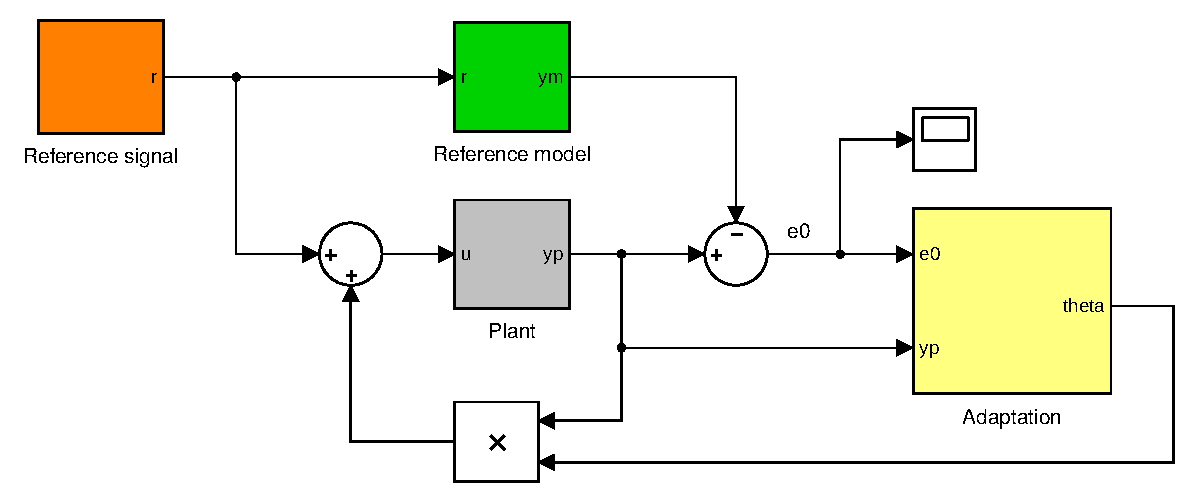
\includegraphics[width=14cm]{figs/blocks/MRAC_111_8_5.eps}
  \caption{Diagrama de blocos do sistema. \quad
  (Model: \HI{\texttt{MRAC-111.mdl}}) }
\end{figure}

%---------------------------------------------------------------------
\bigskip%
\begin{figure}[H]
  \centering
  \includegraphics[scale=0.8]{figs/blocks/plant.eps}
  \caption{Diagrama de blocos da planta.}
\end{figure}

%---------------------------------------------------------------------
\bigskip%
\begin{figure}[H]
  \centering
  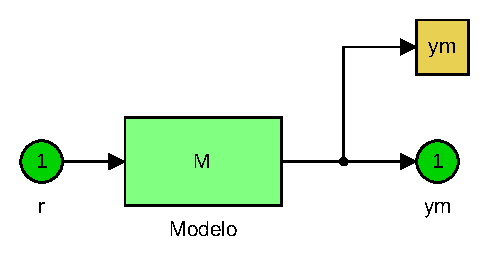
\includegraphics[scale=0.8]{figs/blocks/reference-model.eps}
  \caption{Diagrama de blocos do modelo de refer�ncia.}
\end{figure}

%---------------------------------------------------------------------
\bigskip%
\begin{figure}[H]
  \centering
  \includegraphics[scale=0.8]{figs/blocks/reference-signal.eps}
  \caption{Diagrama de blocos do gerador de sinais de refer�ncia.}
\end{figure}

%---------------------------------------------------------------------
\bigskip%
\begin{figure}[H]
  \centering
  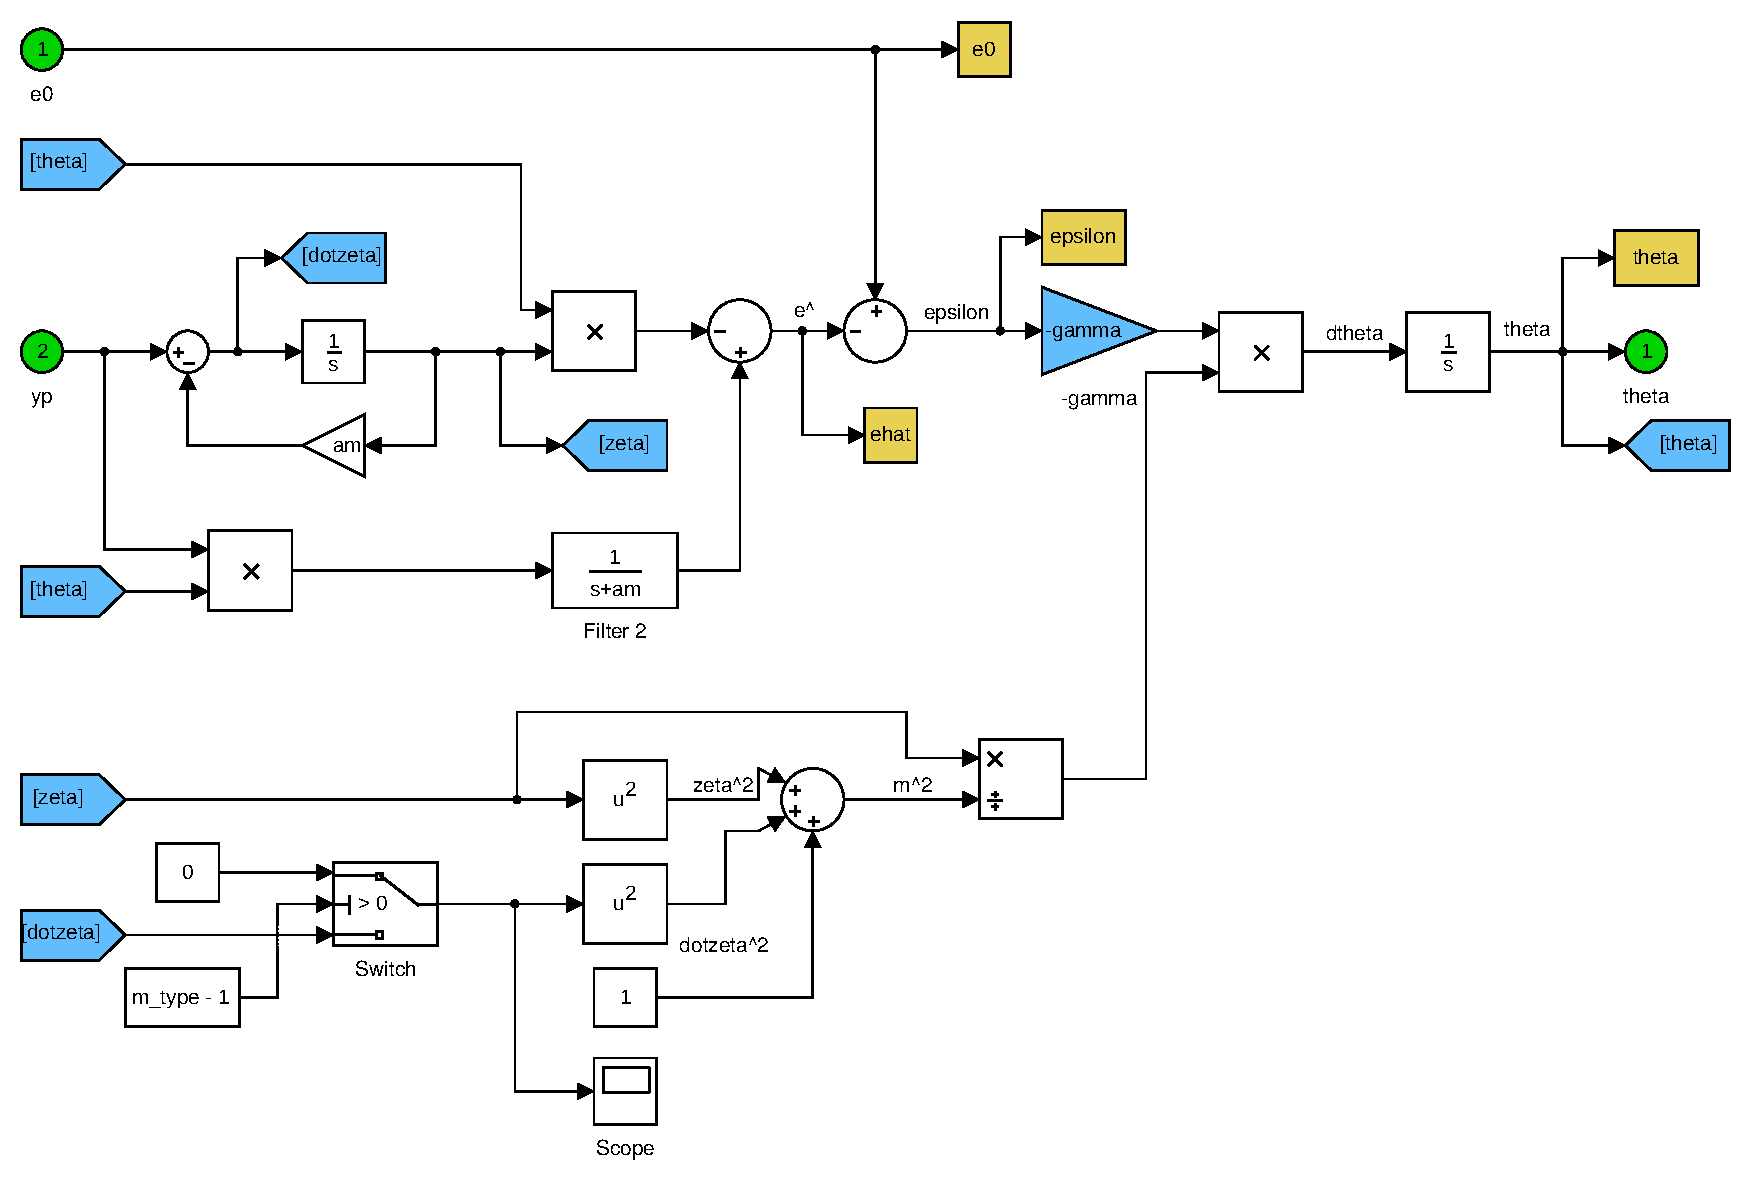
\includegraphics[width=16cm]{figs/blocks/adaptation.eps}
  \caption{Diagrama de blocos da lei de adapta��o.}
\end{figure}